\chapter{Emergence of communities}
\label{ch:communities}

\section{Communities nobody designed}

So far the local rules of this book have explained the \emph{degree} structure of
networks --- their power laws, their clustering hierarchy, their correlations.
This chapter turns to a feature of an altogether different kind: \emph{community
structure}. A community is a group of nodes that are densely connected among
themselves but only sparsely connected to the rest of the network --- a clump
that hangs together. They are everywhere in real data: people fall into social
circles, web pages into topics, proteins into functional modules, each group
talking mostly to itself. Splitting a network into such groups is what
researchers mean by \emph{community detection}, and a network that splits cleanly
is said to have strong community structure.

Where do these communities come from? The usual answer points to differences
between the nodes themselves --- \emph{node heterogeneity}, in the jargon. People
of the same profession or politics, web pages on the same subject, proteins with
the same biological function: nodes of a kind, the story goes, are simply more
likely to link to one another, and that built-in preference is what carves the
network into groups. On this view, communities are stamped onto the network by
properties the nodes carried in from the start.

The thesis of this chapter, following \citet{vazquezcommunities2025}, is that no
such stamp is needed. \emph{Communities emerge from local growth rules even when
every node is identical.} The first hint is decades old: \citet{jin2001} showed
that a social network grown purely by triadic closure --- the friends-of-friends
rule of Chapter~\ref{ch:friends} --- develops communities although its nodes are
all of one type, and the same was later seen in the gene-duplication models of
Chapter~\ref{ch:duplication} \citep{sole2002}. If a featureless local rule
segregates a network into groups all by itself, then community structure joins
preferential attachment and the clustering hierarchy as one more thing that
\emph{emerges} from locality rather than being designed in.

To make that claim sharp we should ask it as a quantitative question, and the
right way to frame it comes from a corner of mathematics called \emph{Ramsey
theory}. Ramsey theory studies how large a random structure must become before
some orderly pattern is forced to appear. Its best-known nugget is a party fact:
in any gathering of six people, there are always either three who all know one
another or three who are all mutual strangers --- order of that kind is
unavoidable once the group is big enough. We will ask the analogous question of
growing networks: given a local growth rule, how large must the network become
before it is virtually \emph{certain} to contain communities? This chapter is, in
effect, a Ramsey theory of community structure in growing networks.

\section{The Ramsey community number}

Before we can measure when communities appear, we need a trustworthy way to
\emph{detect} them, and here some care is required, because the most popular
method can be fooled. That method, \emph{modularity optimization}, looks for the
division of a network that packs the most links inside groups; the trouble is
that it will happily report groups even in a completely random network that has
no real structure at all \citep{newman2006,fortunato2010}. To avoid being
deceived, the work relies instead on two more discerning tools: the
\emph{stochastic block model}, which fits the network to a statistical model of
blocks and keeps only the structure that genuinely earns its keep
\citep{karrer2011}, cross-checked against \emph{Infomap}, which finds groups by
watching where a random walker gets trapped \citep{rosvall2008}. Both, crucially,
report \emph{no} communities in a truly random network.

That last point also supplies the essential control. To be sure a community is
the work of the growth rule and not merely of the degrees, one compares the grown
network against a \emph{rewired} version of itself --- the links shuffled at
random while every node keeps its number of connections (this shuffling is called
the configuration model). If the communities survive the shuffle, they were never
more than an accident of the degrees; if they vanish, they were the doing of the
local rule. For every local model in this chapter, the shuffled version has no
communities at all --- so whatever structure we find is genuinely built by the
dynamics.

\begin{figure}[t]
\centering
\begin{adjustbox}{max width=\linewidth}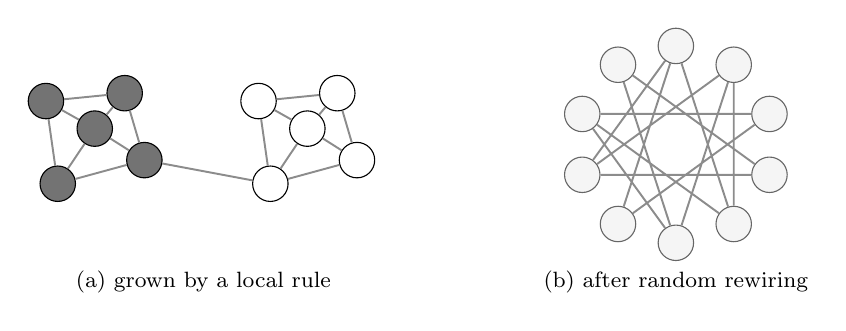
\begin{tikzpicture}[
  nd/.style={circle,draw=black!60,fill=black!4,minimum size=4.5mm,inner sep=0pt},
  cL/.style={circle,draw=black,fill=black!55,minimum size=4.5mm,inner sep=0pt},
  cR/.style={circle,draw=black,fill=white,minimum size=4.5mm,inner sep=0pt},
  lnk/.style={draw=black!45,line width=0.7pt}]
  % panel (a): two communities
  \begin{scope}
    \node[cL] (La) at (0.0,0.9)  {};
    \node[cL] (Lb) at (1.0,1.0)  {};
    \node[cL] (Lc) at (1.25,0.15){};
    \node[cL] (Ld) at (0.15,-0.15){};
    \node[cL] (Le) at (0.62,0.55){};
    \draw[lnk] (La)--(Lb) (La)--(Le) (La)--(Ld) (Lb)--(Lc)
               (Lb)--(Le) (Lc)--(Ld) (Lc)--(Le) (Ld)--(Le);
    \node[cR] (Ra) at (2.70,0.9)  {};
    \node[cR] (Rb) at (3.70,1.0)  {};
    \node[cR] (Rc) at (3.95,0.15) {};
    \node[cR] (Rd) at (2.85,-0.15){};
    \node[cR] (Re) at (3.32,0.55) {};
    \draw[lnk] (Ra)--(Rb) (Ra)--(Re) (Ra)--(Rd) (Rb)--(Rc)
               (Rb)--(Re) (Rc)--(Rd) (Rc)--(Re) (Rd)--(Re);
    \draw[lnk] (Lc)--(Rd);
    \node[font=\footnotesize] at (2.0,-1.4) {(a) grown by a local rule};
  \end{scope}
  % panel (b): rewired, no communities
  \begin{scope}[xshift=6.4cm]
    \foreach \i in {0,...,9}
      \node[nd] (d\i) at ({1.6+1.25*cos(90+36*\i)},{0.35+1.25*sin(90+36*\i)}) {};
    \draw[lnk] (d0)--(d4) (d0)--(d6) (d0)--(d3) (d1)--(d5) (d1)--(d7)
               (d2)--(d6) (d2)--(d8) (d2)--(d5) (d3)--(d7) (d3)--(d9)
               (d4)--(d8) (d5)--(d9) (d6)--(d9);
    \node[font=\footnotesize] at (1.6,-1.4) {(b) after random rewiring};
  \end{scope}
\end{tikzpicture}\end{adjustbox}
\caption{\textbf{Communities emerge from local rules.} (a) A network grown by a
local rule settles into dense communities (two here, one dark gray, one white) joined by
only a few links. (b) Shuffling the links at random while keeping every node's
number of connections destroys the communities --- so the structure was the work
of the rule, not of the degrees alone.}
\label{fig:com-rewire}
\end{figure}

With detection settled, we can pose the question precisely
(Figure~\ref{fig:com-rewire}). The box below states
the two definitions that do the work; both are short, and their meaning is given
in words right after, so the box can be skipped.

\begin{calculation}{the communities likelihood and the Ramsey community number}
For a growth rule $f_G$ that produces a network of $n$ nodes, let a detection
method $f_\kappa$ return the number $\kappa$ of communities it finds. Define the
\emph{communities likelihood} as the probability --- estimated by generating many
networks --- that an $n$-node instance has more than one community,
\begin{equation}
  P_\kappa(n) = \mathrm{Prob}\big\{\, \kappa \ge 2 \,\big\}.
  \label{eq:com-pk}
\end{equation}
The \emph{Ramsey community number} is then the smallest size at which communities
are all but guaranteed, at a confidence $1-\epsilon$ (we use $\epsilon=0.05$,
i.e.\ $95\%$):
\begin{equation}
  r_\kappa = \min\{\, n : P_\kappa(n) \ge 1-\epsilon \,\}.
  \label{eq:com-rk}
\end{equation}
A rule is said to have the \emph{emergent communities property} when such an
$r_\kappa$ exists.
\end{calculation}

In plain terms: $P_\kappa(n)$ is the chance that a network grown to size $n$ has
communities, and the Ramsey community number $r_\kappa$ is the size beyond which
that chance is essentially $(1-\epsilon)100\%$. A \emph{finite} $r_\kappa$ is the fingerprint
of emergence --- grow the network past it and communities are a near-certainty. A
rule for which no such size exists, no matter how large the network, simply does
not make communities on its own. The whole question ``do communities emerge from
this rule?'' thus reduces to ``is $r_\kappa$ finite?''

\section{Local rules grow communities}

We now line up two local rules against two controls. The local rules --- local
search and duplication--split, both met earlier in this book --- have the emergent
communities property; the controls --- reshuffling a network's links, and growing
one with no locality at all --- do not. Holding the four side by side is the whole
argument of the chapter in miniature.

\paragraph{Local search.} The model $\mathrm{LS}(n,d)$ is the search rule of
Chapter~\ref{ch:search} in undirected form \citep{vazquez2001}: each new node
takes a short walk of $d$ steps from a random starting node and links to every
node it visits. It carries preferential attachment and high clustering, and ---
though nothing in the rule ever mentions groups --- the block model resolves clear
communities, with $P_\kappa$ climbing from near zero around $n=10$ to a
near-certain one beyond about $n=100$, and staying there out to a hundred thousand
nodes \citep{vazquezcommunities2025}. Figure~\ref{fig:com-ls} shows one such network.

\begin{figure}[t]
\centering
\begin{adjustbox}{max width=\linewidth}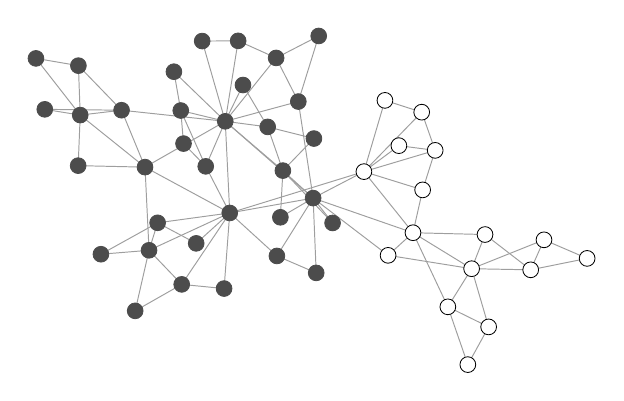
\begin{tikzpicture}[
  netlink/.style={draw=black!38,line width=0.35pt},
  nA/.style={circle,draw=black!70,fill=black!70,line width=0.3pt,inner sep=0pt,minimum size=0.20cm},
  nB/.style={circle,draw=black,fill=white,line width=0.3pt,inner sep=0pt,minimum size=0.20cm}]
  \draw[netlink] (3.520,2.115) -- (2.461,1.926);
  \draw[netlink] (3.520,2.115) -- (4.165,2.451);
  \draw[netlink] (3.520,2.115) -- (4.788,1.675);
  \draw[netlink] (3.520,2.115) -- (4.472,1.388);
  \draw[netlink] (3.520,2.115) -- (2.404,3.090);
  \draw[netlink] (3.520,2.115) -- (3.136,2.464);
  \draw[netlink] (3.520,2.115) -- (3.332,3.341);
  \draw[netlink] (3.520,2.115) -- (3.767,1.799);
  \draw[netlink] (3.520,2.115) -- (3.060,1.380);
  \draw[netlink] (3.520,2.115) -- (3.559,1.165);
  \draw[netlink] (3.520,2.115) -- (3.104,1.871);
  \draw[netlink] (2.461,1.926) -- (4.165,2.451);
  \draw[netlink] (2.461,1.926) -- (2.404,3.090);
  \draw[netlink] (2.461,1.926) -- (1.385,2.508);
  \draw[netlink] (2.461,1.926) -- (2.156,2.518);
  \draw[netlink] (2.461,1.926) -- (1.436,1.452);
  \draw[netlink] (2.461,1.926) -- (3.060,1.380);
  \draw[netlink] (2.461,1.926) -- (1.545,1.801);
  \draw[netlink] (2.461,1.926) -- (1.851,1.019);
  \draw[netlink] (2.461,1.926) -- (2.035,1.540);
  \draw[netlink] (2.461,1.926) -- (2.389,0.966);
  \draw[netlink] (4.165,2.451) -- (4.788,1.675);
  \draw[netlink] (4.165,2.451) -- (4.911,2.219);
  \draw[netlink] (4.165,2.451) -- (5.070,2.721);
  \draw[netlink] (4.165,2.451) -- (4.899,3.206);
  \draw[netlink] (4.165,2.451) -- (4.432,3.356);
  \draw[netlink] (4.165,2.451) -- (4.609,2.781);
  \draw[netlink] (4.788,1.675) -- (4.472,1.388);
  \draw[netlink] (4.788,1.675) -- (5.533,1.218);
  \draw[netlink] (4.788,1.675) -- (4.911,2.219);
  \draw[netlink] (4.788,1.675) -- (5.231,0.734);
  \draw[netlink] (4.788,1.675) -- (5.703,1.652);
  \draw[netlink] (4.472,1.388) -- (5.533,1.218);
  \draw[netlink] (2.404,3.090) -- (1.385,2.508);
  \draw[netlink] (2.404,3.090) -- (1.087,3.231);
  \draw[netlink] (2.404,3.090) -- (3.136,2.464);
  \draw[netlink] (2.404,3.090) -- (2.156,2.518);
  \draw[netlink] (2.404,3.090) -- (3.332,3.341);
  \draw[netlink] (2.404,3.090) -- (2.943,3.019);
  \draw[netlink] (2.404,3.090) -- (3.050,3.895);
  \draw[netlink] (2.404,3.090) -- (2.629,3.551);
  \draw[netlink] (2.404,3.090) -- (2.568,4.112);
  \draw[netlink] (2.404,3.090) -- (1.839,3.227);
  \draw[netlink] (2.404,3.090) -- (2.111,4.109);
  \draw[netlink] (2.404,3.090) -- (1.752,3.720);
  \draw[netlink] (1.385,2.508) -- (1.087,3.231);
  \draw[netlink] (1.385,2.508) -- (0.562,3.169);
  \draw[netlink] (1.385,2.508) -- (1.436,1.452);
  \draw[netlink] (1.385,2.508) -- (0.536,2.527);
  \draw[netlink] (5.533,1.218) -- (5.231,0.734);
  \draw[netlink] (5.533,1.218) -- (5.703,1.652);
  \draw[netlink] (5.533,1.218) -- (5.749,0.479);
  \draw[netlink] (5.533,1.218) -- (6.283,1.204);
  \draw[netlink] (5.533,1.218) -- (6.452,1.585);
  \draw[netlink] (4.911,2.219) -- (5.070,2.721);
  \draw[netlink] (1.087,3.231) -- (0.562,3.169);
  \draw[netlink] (1.087,3.231) -- (0.539,3.797);
  \draw[netlink] (1.087,3.231) -- (0.112,3.242);
  \draw[netlink] (3.136,2.464) -- (3.767,1.799);
  \draw[netlink] (3.136,2.464) -- (2.943,3.019);
  \draw[netlink] (3.136,2.464) -- (3.530,2.871);
  \draw[netlink] (3.136,2.464) -- (3.104,1.871);
  \draw[netlink] (5.231,0.734) -- (5.749,0.479);
  \draw[netlink] (5.231,0.734) -- (5.485,0.000);
  \draw[netlink] (5.070,2.721) -- (4.899,3.206);
  \draw[netlink] (5.070,2.721) -- (4.609,2.781);
  \draw[netlink] (2.156,2.518) -- (1.839,3.227);
  \draw[netlink] (2.156,2.518) -- (1.874,2.807);
  \draw[netlink] (0.562,3.169) -- (0.539,3.797);
  \draw[netlink] (0.562,3.169) -- (0.536,2.527);
  \draw[netlink] (0.562,3.169) -- (0.112,3.242);
  \draw[netlink] (0.562,3.169) -- (0.000,3.889);
  \draw[netlink] (4.899,3.206) -- (4.432,3.356);
  \draw[netlink] (1.436,1.452) -- (1.545,1.801);
  \draw[netlink] (1.436,1.452) -- (1.851,1.019);
  \draw[netlink] (1.436,1.452) -- (0.825,1.402);
  \draw[netlink] (1.436,1.452) -- (1.260,0.683);
  \draw[netlink] (3.332,3.341) -- (3.050,3.895);
  \draw[netlink] (3.332,3.341) -- (3.591,4.174);
  \draw[netlink] (0.539,3.797) -- (0.000,3.889);
  \draw[netlink] (5.703,1.652) -- (6.283,1.204);
  \draw[netlink] (5.749,0.479) -- (5.485,0.000);
  \draw[netlink] (2.943,3.019) -- (2.629,3.551);
  \draw[netlink] (2.943,3.019) -- (3.530,2.871);
  \draw[netlink] (3.050,3.895) -- (2.568,4.112);
  \draw[netlink] (3.050,3.895) -- (3.591,4.174);
  \draw[netlink] (3.060,1.380) -- (3.559,1.165);
  \draw[netlink] (6.283,1.204) -- (6.452,1.585);
  \draw[netlink] (6.283,1.204) -- (7.000,1.349);
  \draw[netlink] (2.568,4.112) -- (2.111,4.109);
  \draw[netlink] (6.452,1.585) -- (7.000,1.349);
  \draw[netlink] (1.545,1.801) -- (0.825,1.402);
  \draw[netlink] (1.545,1.801) -- (2.035,1.540);
  \draw[netlink] (1.851,1.019) -- (2.389,0.966);
  \draw[netlink] (1.851,1.019) -- (1.260,0.683);
  \draw[netlink] (1.839,3.227) -- (1.752,3.720);
  \draw[netlink] (1.839,3.227) -- (1.874,2.807);
  \node[nA] at (3.520,2.115) {};
  \node[nA] at (2.461,1.926) {};
  \node[nB] at (4.165,2.451) {};
  \node[nB] at (4.788,1.675) {};
  \node[nB] at (4.472,1.388) {};
  \node[nA] at (2.404,3.090) {};
  \node[nA] at (1.385,2.508) {};
  \node[nB] at (5.533,1.218) {};
  \node[nB] at (4.911,2.219) {};
  \node[nA] at (1.087,3.231) {};
  \node[nA] at (3.136,2.464) {};
  \node[nB] at (5.231,0.734) {};
  \node[nB] at (5.070,2.721) {};
  \node[nA] at (2.156,2.518) {};
  \node[nA] at (0.562,3.169) {};
  \node[nB] at (4.899,3.206) {};
  \node[nA] at (1.436,1.452) {};
  \node[nA] at (3.332,3.341) {};
  \node[nA] at (0.539,3.797) {};
  \node[nA] at (3.767,1.799) {};
  \node[nB] at (5.703,1.652) {};
  \node[nB] at (5.749,0.479) {};
  \node[nB] at (4.432,3.356) {};
  \node[nA] at (2.943,3.019) {};
  \node[nA] at (3.050,3.895) {};
  \node[nA] at (0.536,2.527) {};
  \node[nA] at (2.629,3.551) {};
  \node[nA] at (3.060,1.380) {};
  \node[nA] at (0.112,3.242) {};
  \node[nB] at (6.283,1.204) {};
  \node[nA] at (2.568,4.112) {};
  \node[nA] at (3.591,4.174) {};
  \node[nB] at (6.452,1.585) {};
  \node[nA] at (1.545,1.801) {};
  \node[nA] at (3.530,2.871) {};
  \node[nA] at (3.559,1.165) {};
  \node[nA] at (1.851,1.019) {};
  \node[nA] at (0.825,1.402) {};
  \node[nA] at (0.000,3.889) {};
  \node[nB] at (7.000,1.349) {};
  \node[nA] at (1.839,3.227) {};
  \node[nA] at (2.111,4.109) {};
  \node[nA] at (2.035,1.540) {};
  \node[nB] at (4.609,2.781) {};
  \node[nA] at (2.389,0.966) {};
  \node[nA] at (1.752,3.720) {};
  \node[nA] at (3.104,1.871) {};
  \node[nA] at (1.260,0.683) {};
  \node[nB] at (5.485,0.000) {};
  \node[nA] at (1.874,2.807) {};
\end{tikzpicture}
\end{adjustbox}
\caption{\textbf{Communities in a local-search network.} An instance of the
local-search model $\mathrm{LS}(n{=}50,d{=}1)$. The stochastic block model
resolves two communities, shown dark gray and white; they emerge even though the
rule treats every node alike and never mentions groups.}
\label{fig:com-ls}
\end{figure}

\paragraph{Duplication--split.} The model $\mathrm{DS}(n,q)$ is the undirected
cousin of the project-schedule rule of Chapter~\ref{ch:projects}: a new node
either copies all of a random node's links (probability $q$) or splits one of its
links in two. This model is the decisive case, because it builds \emph{no
triangles whatsoever} --- duplication makes none, and splitting destroys any that
might form --- and yet communities emerge just as reliably. The lesson is sharp: a
network does not need to be cliquish to have communities. What it needs is
locality, not triangles. Figure~\ref{fig:com-ds} shows an instance: two
communities, and not a triangle in sight.

\paragraph{Degree-preserving randomization.} To be sure the communities are the
work of the local rule and not of the degrees alone, we need a way to wipe out the
local structure while leaving every degree untouched. The \emph{configuration
model}, met when we defined the Ramsey number, does exactly that: it takes a
finished network and reshuffles its links at random, keeping each node's number of
connections fixed but scrambling \emph{which} nodes are joined. Applied to a
local-search or a duplication--split network, this reshuffling destroys the
communities outright --- the randomized versions have no finite Ramsey number at
all (the two ``randomized'' rows in the table below). Whatever the local rules
built, the bare list of degrees cannot sustain.

\paragraph{Barab\'asi--Albert.} Finally, $\mathrm{BA}(n,m)$ --- the canonical
preferential-attachment model --- is our \emph{non-local} control: a growing,
rich-get-richer network in which each newcomer attaches its $m$ links to nodes
drawn from the \emph{whole} graph, never once consulting a neighborhood. Despite
its growth and its rich-get-richer rule it has no emergent communities (the last
row of the table), and the next section is devoted to teasing apart exactly why.

\begin{figure}[t]
\centering
\begin{adjustbox}{max width=\linewidth}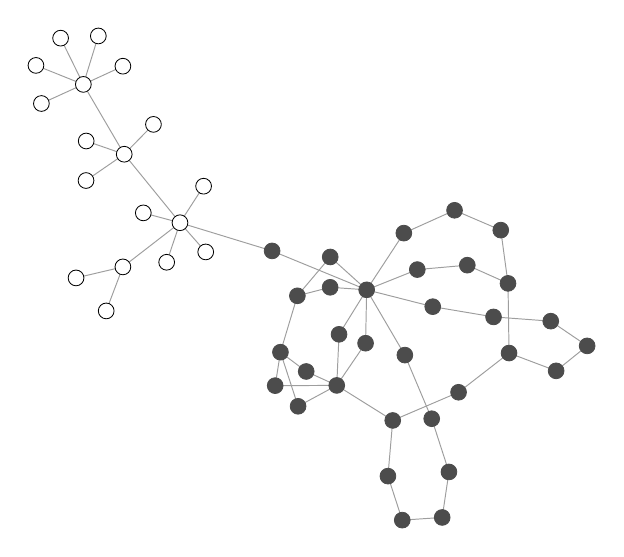
\begin{tikzpicture}[
  netlink/.style={draw=black!38,line width=0.35pt},
  nA/.style={circle,draw=black!70,fill=black!70,line width=0.3pt,inner sep=0pt,minimum size=0.20cm},
  nB/.style={circle,draw=black,fill=white,line width=0.3pt,inner sep=0pt,minimum size=0.20cm}]
  \draw[netlink] (1.363,3.902) -- (1.829,3.777);
  \draw[netlink] (1.829,3.777) -- (2.156,3.406);
  \draw[netlink] (1.829,3.777) -- (2.129,4.241);
  \draw[netlink] (1.829,3.777) -- (1.104,3.216);
  \draw[netlink] (1.829,3.777) -- (1.121,4.647);
  \draw[netlink] (1.829,3.777) -- (1.660,3.275);
  \draw[netlink] (1.829,3.777) -- (2.999,3.419);
  \draw[netlink] (4.531,1.266) -- (3.820,1.711);
  \draw[netlink] (4.531,1.266) -- (4.470,0.559);
  \draw[netlink] (4.531,1.266) -- (5.367,1.624);
  \draw[netlink] (5.159,0.034) -- (5.245,0.612);
  \draw[netlink] (5.159,0.034) -- (4.652,0.000);
  \draw[netlink] (4.200,2.925) -- (5.039,2.711);
  \draw[netlink] (4.200,2.925) -- (4.186,2.247);
  \draw[netlink] (4.200,2.925) -- (4.685,2.096);
  \draw[netlink] (4.200,2.925) -- (3.849,2.360);
  \draw[netlink] (4.200,2.925) -- (3.736,2.957);
  \draw[netlink] (4.200,2.925) -- (4.672,3.645);
  \draw[netlink] (4.200,2.925) -- (3.737,3.342);
  \draw[netlink] (4.200,2.925) -- (2.999,3.419);
  \draw[netlink] (4.200,2.925) -- (4.843,3.182);
  \draw[netlink] (0.892,2.657) -- (1.104,3.216);
  \draw[netlink] (5.039,2.711) -- (5.811,2.581);
  \draw[netlink] (0.792,6.149) -- (0.602,5.534);
  \draw[netlink] (1.104,3.216) -- (0.509,3.076);
  \draw[netlink] (1.121,4.647) -- (0.636,4.313);
  \draw[netlink] (1.121,4.647) -- (0.602,5.534);
  \draw[netlink] (1.121,4.647) -- (1.492,5.026);
  \draw[netlink] (1.121,4.647) -- (0.638,4.815);
  \draw[netlink] (4.186,2.247) -- (3.820,1.711);
  \draw[netlink] (3.820,1.711) -- (3.038,1.708);
  \draw[netlink] (3.820,1.711) -- (3.849,2.360);
  \draw[netlink] (3.820,1.711) -- (3.432,1.888);
  \draw[netlink] (3.820,1.711) -- (3.329,1.446);
  \draw[netlink] (4.685,2.096) -- (5.026,1.288);
  \draw[netlink] (3.320,2.849) -- (3.105,2.133);
  \draw[netlink] (3.320,2.849) -- (3.736,2.957);
  \draw[netlink] (3.320,2.849) -- (3.737,3.342);
  \draw[netlink] (0.602,5.534) -- (0.313,6.121);
  \draw[netlink] (0.602,5.534) -- (1.104,5.765);
  \draw[netlink] (0.602,5.534) -- (0.000,5.775);
  \draw[netlink] (0.602,5.534) -- (0.069,5.291);
  \draw[netlink] (5.245,0.612) -- (5.026,1.288);
  \draw[netlink] (4.470,0.559) -- (4.652,0.000);
  \draw[netlink] (3.105,2.133) -- (3.038,1.708);
  \draw[netlink] (3.105,2.133) -- (3.432,1.888);
  \draw[netlink] (3.105,2.133) -- (3.329,1.446);
  \draw[netlink] (6.008,2.122) -- (5.367,1.624);
  \draw[netlink] (6.008,2.122) -- (5.995,3.007);
  \draw[netlink] (6.008,2.122) -- (6.606,1.896);
  \draw[netlink] (5.478,3.238) -- (5.995,3.007);
  \draw[netlink] (5.478,3.238) -- (4.843,3.182);
  \draw[netlink] (5.995,3.007) -- (5.903,3.683);
  \draw[netlink] (5.811,2.581) -- (6.538,2.527);
  \draw[netlink] (7.000,2.213) -- (6.606,1.896);
  \draw[netlink] (7.000,2.213) -- (6.538,2.527);
  \draw[netlink] (4.672,3.645) -- (5.316,3.935);
  \draw[netlink] (5.316,3.935) -- (5.903,3.683);
  \node[nB] at (1.363,3.902) {};
  \node[nB] at (1.829,3.777) {};
  \node[nB] at (2.156,3.406) {};
  \node[nA] at (4.531,1.266) {};
  \node[nA] at (5.159,0.034) {};
  \node[nA] at (4.200,2.925) {};
  \node[nB] at (0.892,2.657) {};
  \node[nB] at (2.129,4.241) {};
  \node[nA] at (5.039,2.711) {};
  \node[nB] at (0.792,6.149) {};
  \node[nB] at (1.104,3.216) {};
  \node[nB] at (1.121,4.647) {};
  \node[nA] at (4.186,2.247) {};
  \node[nB] at (1.660,3.275) {};
  \node[nA] at (3.820,1.711) {};
  \node[nB] at (0.636,4.313) {};
  \node[nA] at (4.685,2.096) {};
  \node[nB] at (0.509,3.076) {};
  \node[nA] at (3.320,2.849) {};
  \node[nB] at (0.602,5.534) {};
  \node[nA] at (5.245,0.612) {};
  \node[nA] at (4.470,0.559) {};
  \node[nA] at (3.105,2.133) {};
  \node[nA] at (3.038,1.708) {};
  \node[nA] at (6.008,2.122) {};
  \node[nA] at (5.367,1.624) {};
  \node[nA] at (5.478,3.238) {};
  \node[nB] at (0.313,6.121) {};
  \node[nB] at (1.104,5.765) {};
  \node[nA] at (3.849,2.360) {};
  \node[nB] at (1.492,5.026) {};
  \node[nA] at (3.736,2.957) {};
  \node[nA] at (4.652,0.000) {};
  \node[nA] at (5.995,3.007) {};
  \node[nA] at (5.811,2.581) {};
  \node[nA] at (7.000,2.213) {};
  \node[nB] at (0.000,5.775) {};
  \node[nA] at (6.606,1.896) {};
  \node[nA] at (4.672,3.645) {};
  \node[nA] at (3.737,3.342) {};
  \node[nA] at (5.316,3.935) {};
  \node[nA] at (5.026,1.288) {};
  \node[nA] at (2.999,3.419) {};
  \node[nA] at (6.538,2.527) {};
  \node[nA] at (4.843,3.182) {};
  \node[nA] at (3.432,1.888) {};
  \node[nA] at (5.903,3.683) {};
  \node[nA] at (3.329,1.446) {};
  \node[nB] at (0.638,4.815) {};
  \node[nB] at (0.069,5.291) {};
\end{tikzpicture}
\end{adjustbox}
\caption{\textbf{Communities in a duplication--split network.} An instance of the
duplication--split model $\mathrm{DS}(n{=}50,q{=}0.3)$. Two communities (dark gray
and white) again emerge --- even though this rule builds no triangles at all, so the
network is far less cliquish than the local-search one of
Figure~\ref{fig:com-ls}.}
\label{fig:com-ds}
\end{figure}

A few representative Ramsey numbers, based on numerical estimates for $\epsilon=0.05$
\citep{vazquezcommunities2025}, make the pattern concrete:

\begin{center}
\begin{tabular}{lcc}
\hline
Model & $r_\kappa$ (block model) & $r_\kappa$ (Infomap) \\
\hline
$\mathrm{LS}(d=1)$               & $81$   & $222$  \\
$\mathrm{DS}(q=0.5)$             & $98$   & $622$  \\
$\mathrm{LS}(d=1)$, randomized   & ---    & ---    \\
$\mathrm{DS}(q=0.5)$, randomized & ---    & ---    \\
$\mathrm{BA}(m=2)$               & ---    & ---    \\
\hline
\end{tabular}
\end{center}
Every genuinely local rule has a finite Ramsey number --- grow it past a few
hundred nodes and communities are certain. The rules without local structure ---
the bottom three rows, the two reshuffled networks and the Barab\'asi--Albert
model --- have none: the dashes mean communities never become certain, however
large the network. The exact figures differ between the
two detection methods --- there is no single ``true'' definition of a community,
and where the line falls depends a little on how one draws it --- but the
\emph{split} between local rules (finite) and non-local ones (infinite) is the
same either way. Local structure is a necessary condition for communities to
emerge.

\section{When globality fails: the Barab\'asi--Albert model}

The natural control is the Barab\'asi--Albert model \citep{barabasi1999}, the
textbook growing network with \emph{no} locality at all: each newcomer attaches
its $m$ links to nodes chosen from the \emph{whole} network in proportion to
their degree. It has growth and preferential attachment, but no step that ever
looks at a node's neighborhood --- and it does \emph{not} have the emergent
communities property. Its community likelihood rises only to about one-half near
a thousand nodes and then \emph{falls} as the network grows further, never
reaching certainty. The little structure it has comes from the mere age-ordering
of its nodes, not from any local rule, and it washes out at scale.

The boundary case is illuminating. Give the model a baseline ``attractiveness''
$a$, so that a node is chosen with a probability proportional to $a +
k_i/\sum_j k_j$ --- a fixed head-start $a$ on top of the usual degree preference.
This tunes the degree exponent to $\gamma=2+a/m$. Tracking the Ramsey number
across these variants reveals a clean rule of thumb: communities emerge exactly
when the network is \emph{clustered} enough. The Ramsey number falls as the
average clustering coefficient rises, and \emph{diverges} --- communities never
become certain --- as the clustering goes to zero \citep{vazquezcommunities2025}. The standard Barab\'asi--Albert
model sits right at that vanishing point, because its clustering decays toward
zero as it grows (like $(\ln n)^2/n$): the bigger it gets, the fewer short cycles
it has, and short cycles are what local structure is made of. So even here the
principle holds --- where the dynamics happen to generate appreciable clustering
(an \emph{implicit} bit of local structure), communities appear; where clustering
fades, they do not.

\section{How local must ``local'' be?}

If locality is the cause, exactly how local must a connection be to count? Two
dials settle it: the length of the cycles a rule creates, and the distance it
reaches across. Triadic closure closes triangles (cycles of length three); the
duplication--split rule works with squares (length four). To sweep the cycle
length freely, use the \emph{bubble model}: at each step a chain of $L$ new nodes
is added and its two ends are attached to the two ends of a randomly chosen
existing link, creating a fresh cycle of length $L+2$. As $L$ grows --- as the
rule weaves ever longer cycles --- the Ramsey number climbs with it, and steeply:
from $r_\kappa=108$ for the shortest cycles to more than fifty thousand by $L=9$
\citep{vazquezcommunities2025}, as the table below records. The climb is not quite
smooth --- riding on top of it is a regular even--odd alternation, the odd-length
cycles bringing communities on sooner than the even cycles around them, an effect
plainest for the shorter cycles --- but the overall message is unmistakable: short
cycles, tight local feedback, bring communities on soonest.

\begin{center}
\begin{tabular}{ccc}
\hline
$L$ & cycle length $L+2$ & $r_\kappa$ \\
\hline
1 & 3  & 108 \\
2 & 4  & 326 \\
3 & 5  & 246 \\
4 & 6  & 2201 \\
5 & 7  & 752 \\
6 & 8  & 6595 \\
7 & 9  & 2740 \\
8 & 10 & 15863 \\
9 & 11 & 56160 \\
\hline
\end{tabular}
\end{center}

Distance matters just as much. In the bubble model the chain's two ends attach to
nodes that are a single step apart (the ends of one link). Loosen this so the
ends may attach to nodes up to $W$ steps apart, with the chain length fixed at
$L=1$. For $W=1$ communities still emerge with certainty, at $r_\kappa=108$;
stretching to $W=2$ pushes the threshold up roughly tenfold, to $r_\kappa=1090$,
but the communities still come. At $W=3$ --- and likewise if the ends are joined
to nodes picked anywhere at random --- they stop appearing altogether, the Ramsey
number ceasing to exist (the dash in the table) \citep{vazquezcommunities2025}.

\begin{center}
\begin{tabular}{cc}
\hline
$W$ & $r_\kappa$ \\
\hline
1 & 108 \\
2 & 1090 \\
3 & --- \\
\hline
\end{tabular}
\end{center}

For this model, ``local'' means roughly two steps: communities form
when new links reinforce ties among nearby nodes, and dissolve once links are
allowed to leap across the network. This is the whole book's premise made
quantitative. It is not growth, nor preferential attachment, nor even clustering
in the abstract that carves a network into communities --- it is the
\emph{locality} of the rule by which it grew.

\section{Summary}

Community structure, long blamed on built-in differences between nodes, is
instead something that \emph{emerges} from growing a network by local rules, even
when every node is identical. Made precise through the Ramsey community number
$r_\kappa$ --- the size beyond which communities are all but certain --- the
statement is clean: the local rules of earlier chapters (search and
duplication--split) have a finite $r_\kappa$, while their
degree-preserving shuffles, and the non-local Barab\'asi--Albert model, have none.
Triangles are not required (duplication--split makes none and still segregates),
but locality is: communities come soonest for rules that close short cycles
between nearby nodes, and disappear once links may span the whole network. Having
already accounted for degree distributions, the clustering hierarchy, and degree
correlations, this chapter adds community structure to the list of global
patterns that locality alone can explain \citep{vazquez2025}.
